\documentclass{sig-alternate-05-2015}

\makeatletter
\def\@copyrightspace{\relax}
\makeatother
\usepackage{graphicx}
\usepackage{caption}    
\usepackage{subfig} 
\usepackage[T1]{fontenc}
\usepackage{amsmath} 
\usepackage[utf8]{inputenc}

\newcommand{\dd}[1]{\mathrm{d}#1}
\renewcommand*\descriptionlabel[1]{\hspace\leftmargin$#1$}

\begin{document}

\title{Reinforcement Learning in the Game of Othello} 

\subtitle{CS701 Final Project Report}

\numberofauthors{2} % 2 authors in this file

\author{
% You can add or remove blocks as needed.
%
% 1st. author
\alignauthor
Will Ernst\\
       \affaddr{Middlebury College}\\
       \affaddr{Middlebury, VT}\\
       \email{wernst@middlebury.edu}
% 2nd. author
\alignauthor
Ghassan Gedeon Achi\\
       \affaddr{Middlebury College}\\
       \affaddr{Middlebury, VT}\\
       \email{ggedeonachi@middlebury.edu}
}

\maketitle

\begin{abstract}

	\textit{This paper explores the implementation of the temporal-difference learning algorithm TD(\(\lambda\)) to train an Artificial Intelligence agent to play the board game `Othello'. The training strategies compared are: learning from self-play, learning against a fixed opponent, and learning against a random opponent. These training strategies are used on two player types, a constant semi-random player and a decreasingly semi-random player. The players are trained using a multi-layer perceptron neural network, which is updated using the TD(\(\lambda\)) algorithm. Our results show that we found a combination of implementation and parameters for our Neural Network which achieved a strong level of play and was able to quite deceicevly beat an Alpha Beta Search Algorithm}

\end{abstract}


\keywords{CS701; TD($\lambda$); Othello; Reinforcement Learning; Neural Networks}

\section{Introduction}

This paper adapts Gerald Tesauro's TD(\(\lambda\)) algorithm the game of backgammon and implements it for the game of `Othello', or as it is more commonly known `Reversi' [Cite]. The game is played on a $8*8$ board and works by having a `Black' and `White' players take turns placing pieces on the board. The initial board configuration has $4$ pieces, $2$ for each player, placed in the center of the board in a diagonal configuration see [Figure (1)] for a visual representation. In Othello, Black goes first; all subsequent moves by the players  must flank one or more of the opponent's pieces$-$meaning that you must place your piece such that it surrounds one or more of the opponent pieces either vertically, horizontally or diagonally$-$the highlighted tiles in [Figure (1)] illustrate these types of move. Flanked pieces are captured and are replaced with pieces of your own color. The game goes on until one player either has no more valid moves or the board is full. Once the game has ended the player with the most pieces wins. The project was motivated by our interest in getting some experience with the emerging field of machine learning, as well as our interest in developing an agent capable of strong play while being trained completely independently. 

\begin{figure}[h!]
  \includegraphics[width=\linewidth]{stboard.png}
  \caption{Initial Board State for Othello}
  \label{fig:board1}
\end{figure}



We used a Neural Network with $1$ input layer, $1$ hidden layer and $1$ output layer. The input of our network was a vectorized representation of the board state and the output of the network was its associated evaluation. To calculate the output of a given board state, the input is fed through the network. The easiest way to visualize this process is to think of the neurons as node, each of the input neurons is connected to every one of the neurons in the hidden layer, and each of the hidden neurons are connected to the output layer, see [Figure (2)] for simplistic visual representation. Each connections has a corresponding weight, and the output of each neuron is equal to the sum of all the weights multiplied by their input. To normalize and smooth out these connections, we use the sigmoid of these sums, this returns an output between $0$ and $1$ for all neurons in our Network. Once a board state has been fed through the network, we can evaluate its strength based on the final output of the network. It is assumed that the greatest value for all possible moves represent the optimal move for the network.

\begin{figure}[h!]
  \includegraphics[width=\linewidth]{simpleNN.png}
  \caption{A simplistic representation of a Neural Network with 1 hidden layer and 1 output layer}
  \label{fig:simpleNN2}
\end{figure}

At each time step$-$after every move$-$the network calculates the error associated with the given move and back-propagates this error through the network. Back-propagation is the process of updating the weights of the connections to correct for the error. If the output value for the current state is greater than the value for the previous state the network deems the previous move `good'; on the other hand, if the value for the previous state is greater than the value for the current state, the network deems the previous move `bad'. Finally, at the end of each game a pre defined reward is respectively given for a win, loss and tie. This reward is used to calculate final error and is then back-propagated through the network. Further details on how this back-propagation works will be discussed in our Methods section. 

Othello is a deterministic game, unlike Backgammon where dice rolls make it is stochastic. As such, to get our Network to explore new game strategies we had to add a Stochastic element to the TD(\(\lambda\)) algorithm. This element is called the exploration rate (\(\epsilon\)), and determines how often our Network will explore moves that are not the expected to be optimal.

In this project, we have devised two types of Network with distinct implementations of the exploration rate. The first of these Network, which we named NN-Fixed has a fixed exploration rate. The second of these Networks, this one called NN-Decreasing has an exponentially decreasing exploration rate. The analysis of these two-distinct implementation is our project's main contribution, and sheds some light on the optimal implementation of reinforcement learning in a deterministic environment.

Our second contribution is seeing how each of these networks perform with different Lambda (\(\lambda\)) values. The lambda value determines the rate of decay in error correction for previous time steps. A \(\lambda\) $= 0.0$ means that no feedback occurs beyond the current time step, and a $\lambda  = 1.0$ means that feedback occurs without decay arbitrarily far back in time. After some testing, we found that high lambda values yielded the best results, so we chose to test the extreme case $\lambda  = 1.0$ vs a slightly less drastic case $\lambda  = 0.9$.

Our third contribution is seeing how the network learns versus various opponent. For this purpose, we created 3 additional opponent against which our network would train against. These opponents are: (1) a fully \emph{Random} agent whose moves are selected randomly, (2) a \emph{Positional Value} opponent, where tiles have a hardcoded value based on how good or bad they are in traditional play \cite{van2013reinforcement}, (3) an AI agent using the \emph{Alpha-Beta} search. Unfortunately, Alpha-Beta proved to be extremely slow even at a depth of $2$, so we chose to only use it as a means of testing our final networks. Thus, both NN-Fixed and NN-Decreasing were trained against opponents (1) and (2), as well as being trained against themselves, and each of these combinations was test with $\lambda  = 1.0$ as well as $\lambda  = 0.9$ . An analysis of these contributions will be covered in our Results section where we evaluate the performance of the various combination of Network types, lambda values and opponent type. All networks were trained for $125,000$ games, and we used their performance against a random agent for $500$ games was used as a measure of strength $-$this choice will be explained in the Methods section. Additionally we used the score of our network against (2) \emph{Positional-Value} agent and (3) \emph{Alpha-Beta} agent as a gauge of performance over time. 

Our final contribution is an implementation of a user-friendly GUI interface for the Game, where the user can choose to play against any of our trained Neural Network, or any of the other agents that we created. As of now the selection of opponent is code based, but in the future we are hoping to create a full fledged web application where the user can select the opponent of choice from a drop down menu. 



\section{Related Work}

\subsection{TD-Gammon}
The work of this paper was motivated by Gerald Tesauro's TD-Gammon. TD-Gammon, developed in 1992, is a backgammon program that uses an artificial neural network trained by the TD(\(\lambda\)) algorithm. The program was a major success at the time, and led to new developments in backgammon strategy and theory.

The program used a standard multilayer perceptron network as a function approximator for the probability of the black player winning at a certain state. The network uses the the TD(\(\lambda\)) backpropagation algorithm to update its weights. The goal of the weight updates, as it is with most temporal difference learning algorithms, is to minimize the temporal-difference error. This error is the difference of the neural network output in time $t+1$ and the neural network output in time $t$. 

The TD gammon program runs as follows: at each timestep the program calculates each possible move using a one ply look ahead (this means that it only looks one move ahead of its current state). Those moves are vectorized into neural network inputs and are fed into the network. The feedforward output of the network is a vector of four outputs corresponding to the four possible outcomes of either White or Black winning either a normal win or a gammon. Due to extreme rarity, triple gammon end games were not included. The best value for the player is chosen and the weights are updated using TD(\(\lambda\)). When a game is over, instead of calculating a new move, the board state is assigned a value of $0$ or $1$ for white winning the game or black winning the game, respectively. 

During training, the neural network itself is used to select moves for both sides. With this training paradigm, the program only learns from what its own moves are. This paradigm is used throughout the entire training, even at the beginning when the weights of the network are random. Although at the beginning the network has no sensible strategy, it is improved through self play as it observes successful sequences of moves.
The results of TD-Gammon were impressive. Although the initial state of the program had no knowledge of the game, it was able to develop basic strategies for the game early on, such as hitting the opponent, playing safe, and building new points. This was observed after just a few thousand games. After several tens of thousands of training games, more sophisticated strategies were observed. In terms of the setup of the network, it was noted that substantial improvements in performance were observed when the size of the network and amount of training experience increased.
In examination of the weights from the input to hidden layer, the network revealed interesting spatially organized patterns of positive and negative weights, corresponding to useful features of the game. This implies that TD-Gammon was capable of automatic ``feature discovery'', which is one of the original goals of game learning research.

To evaluate the success of the program, it was tested against world-class human opponents. The first iteration of the program, version $1.0$, achieved respectable results against Bill Robertie, Paul Magriel, and Malcolm Davis, (ranked 11th in the world at the time), net loss of $13$ points and an average loss rate of about $1$ quarter point per game. Version $2.0$ of the program added more training iterations and a 2-ply look ahead. Playing Kent Goulding, Kit Woolsey, Wilcox Snellings, former World Cup Champion Joe Sylvester, and former World Champion Joe Russell, the program had a net loss of only $7$ points. Version $2.1$ of the program achieved near parity to Robertie, who only managed to beat the program in the last game resulting in a narrow $1$-point victory.

\subsection{Othello research}

Previous research has been done on using reinforcement learning (RL) algorithms to solve the game Othello. Work by Ree et al. explores Othello with three learning strategies: Learning by self-play, learning from playing, against a fixed opponent, and learning from playing against a fixed opponent while learning from the opponent's moves as well. Their work examines three commonly used RL algorithms, Q-learning, Sarsa, and TD-learning. Results from their testing show that each algorithm has its own optimal training strategy. Q-learning and Sarsa performed best when trained along with a fixed opponent, while TD-learning performed best when trained through self-play. Additionally they found that learning from the opponent's as well as the player?s own moves moves generally performed worse than just learning from the player's own moves

\section{Methods}

\subsection{Network Layers}
 
To implement the TD(\(\lambda\)) algorithm we used a Neural Network with an input layer with $64$ neurons, one hidden layer with $50$ neurons and an output layer with single neuron. The output neuron was used to evaluate the board state.

Since Neural Networks require vector inputs we converted our $8*8$ board state into a vector of size $64$ with value of $0$, $1$ and $-1$, which respectively correspond to an empty tile, tile containing a Black piece and a tile containing a white piece.

The hidden layer is comprised of $50$ neurons. This choice comes from testing various implementations of the network, and picking the network that showed strong learning performance while remaining not too computationally demanding. Since each additional hidden neuron adds 65 connections$-$$64$ to the input layer and $1$ to the output layer$-$the computational cost of adding one or more is rather steep.
 
\subsection{Sigmoid Neurons}
\begin{figure}[h!]
  \includegraphics[width=\linewidth]{neuron.png}
  \caption{Visual representation of a neuron in a Neural Network}
  \label{fig:neuron4}
\end{figure}
 
        	Perceptron's were developed in the 1950's and 1960's by a scientist named Frank Rosenblatt, who was inspired by the earlier work of Warren McCulloch and Walter Pitts. These are the most basic type of Neurons you can use in a Neural Network. Perceptron's take inputs with corresponding weights, and output a value of $0$ or $1$. This work by setting a threshold, and output corresponding value for outputs below or above the determined threshold. [Figure (3)] and [Equation (1)] show the basic functioning of a Perceptron \cite{rosenblatt1958perceptron}.

\begin{equation}
output =
\left\{
	\begin{array}{ll}
		0, & \mbox{if } \sum_j  w_j x_j \leq Threshold \\
		1, & \mbox{if } \sum_j  w_j x_j > Threshold
	\end{array}
\right.
\end{equation}

\begin{equation}
output = \frac{1}{1+e^{-z}}
\end{equation}



	
	The issue with perceptron's is that small changes in the weights can cause major changes in the output of the neuron, as such Perceptron networks for complicated task can be very hard to train. With that in mind, we chose to use Sigmoid Neurons for our implementation of the networks. Visually these look the same as Perceptron [Figure(3)], but the output of the neuron is passed into a sigmoid function [Equation (2)], where $z$ is the sum of the weights multiplied by the input of the neuron. This returns a value between $0$ and $1$. A graphical representation of the outputs of Perceptron vs Sigmoid Neurons can be seen in [Figure (4)].
	
\begin{figure}[h!]
\centering
\subfloat[Percetron output value]{\hspace*{-.5cm}\includegraphics[width=0.5\linewidth, keepaspectratio]{sigmoid.png}\label{fig:subfig1}}
\subfloat[Sigmoid output value]{\includegraphics[width=0.5\linewidth, keepaspectratio]{perceptron.png}\label{fig:subfig2}}
\caption{Different between Perceptron and Sigmoid output}
\label{fig:graph5}
\end{figure}
	
\subsection{TD(\(\lambda\))}

	The TD(\(\lambda\)) algorithm was designed by Richard Sutton in 1988. Most prediction learning methods at the time assigned credit by means of the difference between a predicted and actual value. Sutton?s method, on the other hand, assigned credit by means of the difference between temporally successive predictions [2]. The network weights are updated according to the following rule [3]:
	
\begin{equation}
w_{ij}^{t+1} = w_{ij}^t + \alpha  \sum\limits_{k\in O} (P_k^{t+1} - P_k^{t}) e_{ij}^t 
\end{equation}

Where
\begin{description}
\itemsep0em 
\item [w_{ij}^{t+1}] is the weight at time $t$ from node $i$ to $j$
\item[\alpha] is the learning rate parameter
\item[O] is the `Set' of outputs given by the output layer
\item[P_k^{t}] is output value of the output node $k$ at time $t$
\item[e_{ij}^t] is the eligibilty trace matrix at time t
\end{description} 
\
	
The weights are updated through this method in every turn of the game. The TD error is calculated as: 

\begin{equation}
 \sum\limits_{k \in O} (P_k^{t+1} - P_k^t)
\end{equation}

In the case of Othello, there is only one output node, so the summation is not necessary. In this paper?s othello implementation, endgame states pass in a hardcoded of $0$ for white winning, $0.5$ for a tie, and $1$ for black winning. The goal of the program is to minimize this error. If it does so, then the algorithm will have found a sequence of moves that perfectly predicts the outcome of the game. The learning rate, $\alpha$, is a weight parameter for the error to determine how much the total error will affect the weight change. The eligibility matrix is used in the algorithm to determine which weights are ?eligible? to be updated. When TD error occurs and learning needs to be done, only eligible states are assigned credit for the error. This matrix keeps a running memory of every credit assignment that has occurred in the training. The matrix is calculated as follows[3]:

\begin{equation}
e_{ijk}^t = \sum_{n=1}^{t} \lambda^{t-n} \frac{\partial P_k^n}{\partial w_{ij}^n}
\end{equation}

Where
\begin{description}
\itemsep0em 
\item [\lambda] is the decay parameter for the eligibility matrix
\end{description} 
\

The eligibility matrix is running sum of the previous credit assignments in the network [1]. Previous assignments are decremented at each timestep by the value lambda, so that credit assignments early in training have less of an effect on current credit assignments. The credit assignment is based on a matrix of partial derivatives of the network output with respect to each weight. This determines how much the weight affects the output of the network, and thus how much credit it should get for the error. These partial derivatives are calculated as follows[3]:

\begin{equation}
\hspace*{-.5cm}\frac{\partial P_k^n}{\partial w_{ij}^n} = \delta_{kj}^{t+1} y_i^{t+1}
\end{equation}
\begin{equation}
\hspace*{-.5cm}\delta_{ki}^{i}= \frac{\partial P_k^t}{\partial s_{i}^t} =
\left\{
	\begin{array}{lll}
		y_{i}^{t} (1 - y_{i}^{t}), & \mbox{if } k = i \\
		0 & \mbox{if } k \in  O \text{ and } k \neq i\\
		\sum_{j} \in FO_i \frac{\partial P_k^t}{\partial s_{j}^t} \frac{\partial s_j^t}{\partial y_{i}^t} \frac{\partial y_i^t}{\partial s_{i}^t}\\ =  
		\sum_{j} \in FO_i \delta_{kj}^{t} w_{ij}^{t} y_i^t (1 - y_i^t) & \mbox{otherwise}
	\end{array}
\right.
\end{equation}

Where:
\begin{description}
\itemsep0em 
\item [\delta_{ki}^i] is the error at node $j$
\item[y_i^t] is the output of node $i$  at time $t$ (where $i$ is in the layer before $j$)
\end{description} 
\


From these equations, we can see that the final change for each weight is the a weighted temporal difference error again weighted by how much credit that weight has in the final outcome. The inclusion of a lambda value is considered a bridge between one step TD and Monte Carlo methods. For $\lambda=0$, only the current credit assignment is factored into the weight update, while for $\lambda=1$, all previous credit assignments are equally factored into the weight update. Setting $\lambda$ to a value between $0$ and $1$ gives the result algorithm a mix of both approaches.

Learning and Training:
To teach the network, multiple games are played. For the results presented in this paper, the network was trained with $125,000$ games. Each epoch of training runs as follows:

\begin{enumerate}
\itemsep0em 
\item While $(iterations < total iterations)$
\item  \hspace*{.5cm}\text{If black move:}
\item  \hspace*{1cm}\text{Move and learn}
\item  \hspace*{.5cm}\text{If white move:}
\item   \hspace*{1cm}\text{Move and learn}
\end{enumerate}


Note that with each game, the eligibility matrix is reset, but the weights of the network are not. This is because the eligibility matrix is supposed to keep track of previous moves in the game. For all games, the move in one game is independent of the moves of another, so we do not want to eligibility matrix remembering from past games. In this implementation of TD($\lambda$), while playing a game each move represents a time $t$. At each move the program executes the following:


\begin{enumerate}
\itemsep0em 
\item Observes the current state $s^t$
\item  If $s^t$ is endgame:
\item  \hspace*{.5cm}\text{Set  $s^{t+1} = 0$ if white wins, $s^{t+1} = 0.5$ if tie}, \\  \hspace*{.5cm}\text{$s^{t+1} = 1$ if black wins}
\item   Else:
\item   \hspace*{.5cm}\text{Given $s^t$, the program calculates $A$} \\  \hspace*{.5cm}\text{the possible afterstates of $s^t$}
\item   \hspace*{.5cm}\text{For each $a$ in $A$:}
\item  \hspace*{1cm}Vectorize $a$ into an input for NN
\item \hspace*{1cm}The NN calculates the output of the of $a$
\item \hspace*{1cm}Set $a$ to $s^{t+1}$ if it has the greatest output value
\item   \hspace*{.5cm}Vectorize $s^t$
\item   \hspace*{.5cm}Place a piece on the board in the \\ \hspace*{.5cm} position corresponding with state $s^{t+1}$
\item   Given $s^t$ and $s^{t+1}$, run TD( $\lambda$) to adjust the weights
\end{enumerate}


\subsection{Player Types}
\emph{Neural Network} -- This player is the standard neural network player. It decides its moves based on the neural network output. We found that this player did not train the network well during self play. In training, this player does a poor job at exploring a wide variety of different states. This is because Othello lacks a stochastic element. So, when a network trained by this player was given a state that it had not seen before, it performed poorly. This is the player used for testing the neural network.

\emph{Semi Random Neural Network} -- This player decides its moves based on the neural network only a preset percentage of the time and moves randomly otherwise. The benefit of this player in training is that it has a stochastic element that the Neural Network player does not. To implement this, at each move a random number is selected. If the random number is below some threshold, then the player moves based on the neural network and moves randomly otherwise. This player is mainly used in training, and shows better training results than the Neural Network player.

\emph{Decreasingly Random Neural Network} -- This player decides its moves based on the neural network only an increasing percentage of the time and moves randomly otherwise. This player has similar benefits to the Semi Random Neural Network player, but reinforces more of its moves in later iterations of training. The threshold for the randomness is calculated by an exponential function:

\begin{equation}
T = (1-a) * e^{10 * \frac{(i-n)}{i} }+ a
\end{equation}

Where:
\begin{description}
\itemsep0em 
\item [t] is the threshold 
\item [a] is the initial threshold
\item [i] is the current iteration
\item [n] is the total number of iterations
\end{description} 
\
At the point when $i = n$, the threshold is $1$ and chooses only from the neural network.

\begin{figure}[h!]
  \includegraphics[width=\linewidth]{e-rate.png}
  \caption{Graphical Representation of the exponentially decreasing learning rate}
  \label{fig:neuron4}
\end{figure}


\emph{Random} -- This player decides all its moves randomly. This player is mainly used in testing. Because Othello has no stochastic element, it is difficult to test a trained neural network against non-stochastic players. In these cases of testing, the same game is played every time. With this player, a different game is played in each round of testing so a more accurate win percentage for the network can be calculated.

\emph{Position Values} -- This is a fixed player with a heuristic value assigned to each of the 64 board tiles. It makes its moves based on the maximum tile value of the possible moves. This player is mainly used in testing.

\emph{Greedy} -- This player makes its moves in order to maximize its score. It uses a one ply look ahead to determine which move is best. This player is mainly used in testing.

\emph{Alpha-Beta} -- This player implements the alpha-beta pruning algorithm to its best possible move. The alpha-beta pruning algorithm is a tree search algorithm that minimizes the number of nodes visited in a minimax tree. It is able to forecast possible board states for $k$ timesteps in the future. It selects the move that maximizes its score at state$^{t+k}$, assuming that the other player also moves to maximize its score. This player is mainly used in testing.


\begin{itemize}

\item The Source Code for our project can be found at the following link \emph{https://github.com/wernst/td-othello}
\item The Repository also contains a Subset of the Networks we saved during training, a text file containing the <$Iterations$>$<$Win$ \$Percentages$>  during training for the respective networks, and finally vectorized version of the graphs found in the Results Sections. 

\end{itemize}

\section{Results}
	In the following section we will analyze the learning performance of (1) the implementation of a exponentially decreasing exploration rate as opposed to a fixed exploration rate, (2) we will look at the effect of setting $\lambda = 0.9$ vs. setting $\lambda = 1.0$ and (3) we will look at how our Self-trained Neural Networks performed against our strongest competing Agents \emph{Alpha-Beta} and \emph{Positional-Value}. Finally, (4) we will briefly cover GUI applet that we have developed for users to have a convenient interface which they can use to play against the agent of their choice. Our best implementations reached performances against a random agent of around $90\%$.



\subsection{NN Dec vs NN Fixed}
	Looking at [Figure (6) and Figure (7)], we see very similar patterns in learning for the two different types of network. The results are so similar that it without looking at the Title of the graph I would be unable to distinguish the two. Given the implementation of the exponential exploration decay, we were expecting the networks to behave very similarly until we reach a game $~80,000$, at which time the exploration rate would start decreasing. We had initially hypothesized that when this happened $NN-Decreasing$ would start refining its weights to discover subtler patterns in play style that $NN-Fixed$ would be unable to find. This, however did not happen. In both models, and against all opponents, we saw very similar win percentages.
	There is one aspect small difference in the models that is quite interesting, but somewhat hard to spot. If we carefully look at the difference in win percentages between [Figure (6b)] and [Figure (7b)], specifically for the $red$ line representing self-play, we notice that the line in [Figure (7b)] is much smoother than [Figure (6b)] and this starts right around the $~80,000 games$. This is likely due to the exploration going down and the Network converging towards its final (and ideally optimal) weight configuration. Overall the decreasing exploration rate does not seem to provide too much of a benefit, however if a modified form of this decaying exploration rate were implemented right after the network reaches its maximum win percentage, it could prevent the network from experiencing the sharp dips that can be seen throughout the training. This theorized $adaptive$ exploration rate $\epsilon$ is one possible avenue for future research.

\begin{figure}[p]
\centering
\subfloat[NN-Fixed with Lambda 0.9]{\hspace*{-0.8cm}\includegraphics[width=0.66\linewidth, keepaspectratio]{NN-Fixed-9.png}\label{fig:subfig1}}
\subfloat[NN-Fixed with Lambda 0.9]{\includegraphics[width=0.66\linewidth, keepaspectratio]{NN-Fixed-1.png}\label{fig:subfig1}}
\caption{Graphs for Neural Network with Fixed Exploration Rate}
\label{fig:graph5}
\end{figure}


\subsection{Lambda Value Choice}
During the course of training, both Networks$-NN-Decreasing$ and $NN-Fixed-$ with $\lambda = 0.9$ performances suffered right around reaching the $50,000$ iteration mark, see [Figure (6)] and [Figure (7)]. This decrease in performance seems to happen right after the network reached optimal performance, but our Networks with  $\lambda = 1.0$   didn't seem to suffer from the same issue. During the period of decline, the values of our networks with $\lambda = 0.9$ approached $1$. By the end of training, the evaluation of almost every board state would output a value $> 0.99$. Although we are unsure of exactly why this occurs, we did notice that this pattern occurred earlier with larger $\alpha$ values. Although the goal of the TD($\lambda$) algorithm is to converge to the global minimum of the function approximator, this convergence has only been proven for linear networks and linearly independent sets. In the general case, there is no guarantee that the algorithm will converge even to a local minimum [6]. This finding seems to suggest that for our implementation of the Neural Network a $\lambda = 1.0$ is optimal, but as we experienced over the semester, working with Neural Networks can be tricky. We did not notice the issue with a $\lambda = 0.9$ until our final run, specifically because this convergence only happened fairly late into the training.

\begin{figure}[p]
\centering
\subfloat[NN-Decreasing with Lambda 0.9]{\hspace*{-0.8cm}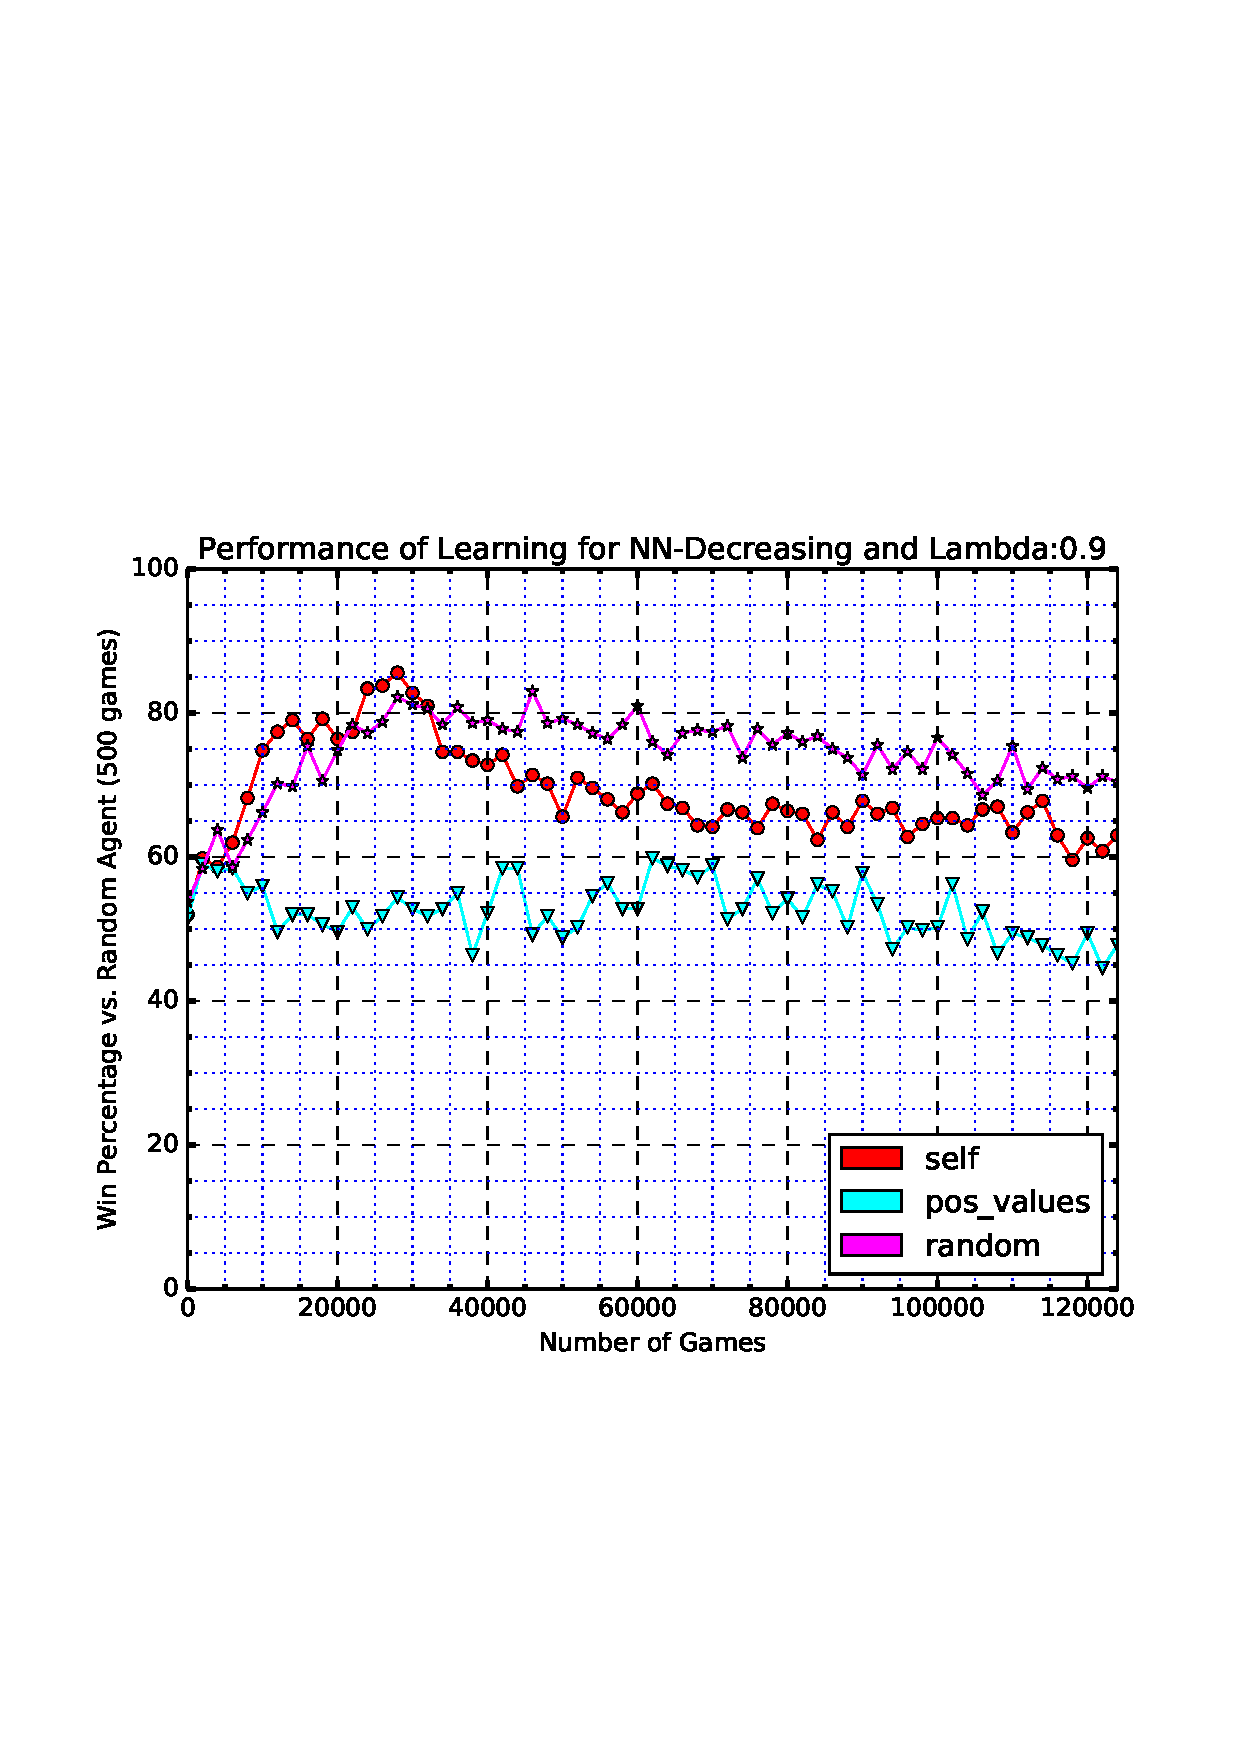
\includegraphics[width=0.66\linewidth, keepaspectratio]{NN-Decreasing-9.png}\label{fig:subfig1}}
\subfloat[NN-Decreasing with Lambda 0.9]{\includegraphics[width=0.66\linewidth, keepaspectratio]{NN-Decreasing-1.png}\label{fig:subfig1}}
\caption{Graphs for Neural Network with Decreasing Exploration Rate}
\label{fig:graph5}
\end{figure}


\subsection{Opponent Types}

	Having established that the $\lambda = 0.9$ causes a detrimental form of convergences in our network, let us now turn our attention back to [Figures (6b)] and [Figure (7b)] to examine the way that the various opponents it trained against affected the Learning Rate. 

\emph{Positional-Value} $-$ Immediately it becomes clear that the network struggles to learn when playing against Positional Value. We had expected that the network would have a hard time beating the agent in the early stages of the game, but we have expected the network (Especially $NN-Decreasing$) to eventually find a weight combination that would allow it to defeat the $Positional-Value$ agent and start learning from playing against it. However, we notice that the performance against $Random$, stagnates around or even below the $50\%$. When we examined the output, we noticed that $Positional-Value$ was winning a significant percentage of the games, which means that neither of our NN were receiving any reward and as such the network was unable to optimize its weight to find a combination that worked best.

\emph{Random} $-$ We were rather surprised at how well our network learned from a fully random opponent. We had not expected that our Neural Networks would learn almost as well against a fully random opponent, as it would against itself. This seems to confirm that high exploration rate allow for quicker learning. It should be noted that in the latter stages of training, the Networks training against a random opponent experienced more spikes and dips in learning that those learning from self-play.

\emph{Self-Play} $-$ as we had expected this showed the best results, reaching a win percentage against Random of around $90\%$. Since this model seemed worked best, we decided to conduct  further experiments and displayed our Networks score vs. both the \emph{Positional-Value} agent, and \emph{Alpha-Beta}  with a max depth of $4$ at various intervals in our training, see [Figure (8)] and [Figure (9)]. In Othello the score can quickly switch since a single move can cause a significant of the board to switch colors. As such, scores are not always the best indicator of learning, but we were curious to see if we noticed any patterns in the data. It should be noted that the $32$-point threshold-indicated by the blue line in the figures$-$ are not a hard minimum on winning scores, as one can win with less than the threshold if he still controls the most number of pieces on the board and the opponent is out of moves. However, in our experience this happened very rarely, and we decided that the potential information loss was still worth the risk. Unfortunately, no subtle pattern emerged, but on a general case, we noticed that our data-points were generally above the $32$-point threshold against $Alpha Beta$, which we were quite impressed with. We theorize that our models moves are much superior to $Alpha-Beta$ in the early games, since $Alpha-Beta$ has the advantage of looking $4$ moves ahead during the end game. 

	Against \emph{Positional-Value} [Figure (9)], the results were quite poor, and this seems to further reinforce what seemed to be true in training, which is that \emph{Positional-Value} is a very strong opponent, which is rather suprising since it simply uses hardcoded inputs.

\begin{figure}[p]
\centering
\subfloat[NN with Lambda 0.9 vs. Alpha-Beta]{\hspace*{-0.8cm}\includegraphics[width=0.66\linewidth, keepaspectratio]{Alpha-Beta-9.png}\label{fig:subfig1}}
\subfloat[NN with Lambda 1.0 vs. Alpha-Beta]{\includegraphics[width=0.66\linewidth, keepaspectratio]{Alpha-Beta-1.png}\label{fig:subfig1}}
\caption{Score of Self-Trained Neural Networks vs. Alpha-Beta}
\label{fig:graph5}
\end{figure}

\subsection{GUI implementation}
	The final contribution that we are making with this paper, is a user-friendly environment in which the player can play against an agent of his choice. The Layout of the applet can be seen in [Figure (10)] \textbf{ADD IMAGE BELOW IF YOU CAN WILL}. We hope to be able to get the applet online soon. Once this happens, the applet's url will be linked from the following addresses:

\begin{itemize}
\itemsep0em 
\item http://www.cs.middlebury.edu/~wernst
\item http://www.cs.middlebury.edu/~ggedeonachi
\end{itemize}


\begin{figure}[p]
\centering
\subfloat[NN with Lambda 0.9 vs. Positional-Value]{\hspace*{-0.8cm}\includegraphics[width=0.66\linewidth, keepaspectratio]{Pos-Val-9.png}\label{fig:subfig1}}
\subfloat[NN with Lambda 1.0 vs. Positional-Value]{\includegraphics[width=0.66\linewidth, keepaspectratio]{Pos-Val-1.png}\label{fig:subfig1}}
\caption{Score of Self-Trained Neural Networks vs. Positional-Value}
\label{fig:graph5}
\end{figure}

\begin{figure}[h!]
  \includegraphics[width=\linewidth]{stboard.png}
  \caption{Initial Board State for Othello}
  \label{fig:board1}
\end{figure}




\section{Discussion}

In this project we compare two  $\lambda$ values ($0.9$ and $1.0$) in their ability to train an Othello player using the TD($\lambda$) algorithm. We found that both values worked best training with self-play. Using self play as the training paradigm, $\lambda  = 1$ worked best for our TD($\lambda$) implementation on training an Othello player. This version of the algorithm is most similar to Monte Carlo methods [1].

For future work with respect to our implementation, we would like to continue to explore combinations of ? values, ? values, network setups, and randomness to determine which results in the best training inputs. Using more advanced network techniques, such as changing of ? values and ? values through the training process is another possibility. We also would like to determine what caused our network during training to inflate all its outputs toward $1,$ when $? < 1$. In general, we feel that this method of learning could be expanded to number of board games.


%ACKNOWLEDGMENTS are optional
\section{Acknowledgments}

This section is optional; it is a location for you to acknowledge grants,
assistance, etc. For example, this report template was adapted from Prof.~Christman.

\bibliographystyle{abbrv}
\bibliography{references}  % references.bib is the name of the BibTex file

\end{document}
